% ===================================================================================================
%                                                 |                                                 |
%                                                 |                                                 |
% -------------------------------------------- SECTION ---------------------------------------------|
%                                                 |                                                 |
%                                                 |                                                 |
% ===================================================================================================
\section{Use case: Smart factory}
\begin{figure*}[!h]
	\centering
	\hspace*{\fill}
	\subfloat[]{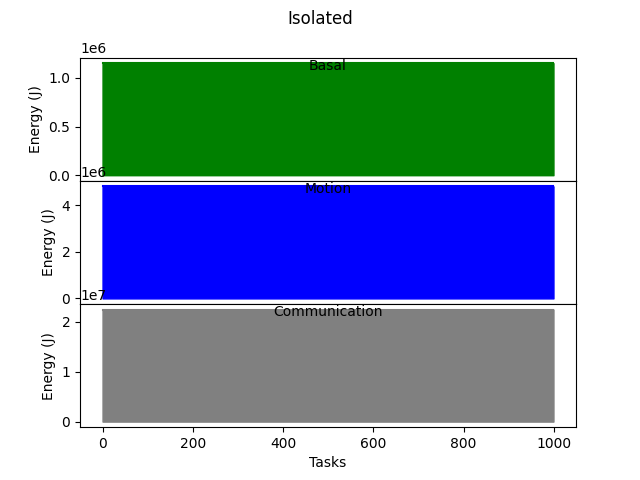
\includegraphics[width= 0.90\columnwidth]{fig/isolated_corrected.png} \label{fig:iso_energy}}
	\hfill
	\subfloat[]{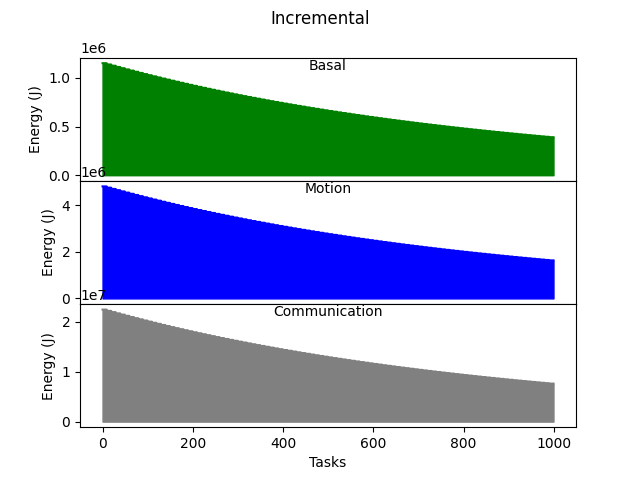
\includegraphics[width= 0.90\columnwidth]{fig/incremental_corrected.png} \label{fig:itl_energy}}
	\hspace*{\fill}
	\\%[-2ex]
	\hspace*{\fill}
	\subfloat[]{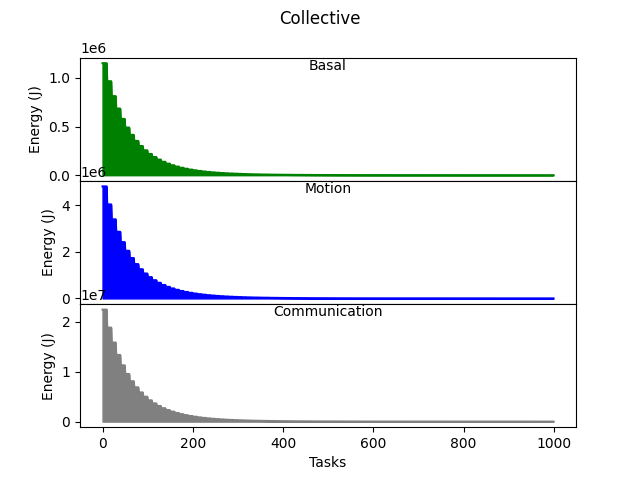
\includegraphics[width= 0.9\columnwidth]{fig/collective_corrected.png}\label{fig:cl_energy}}
	\hfill    
	\subfloat[]{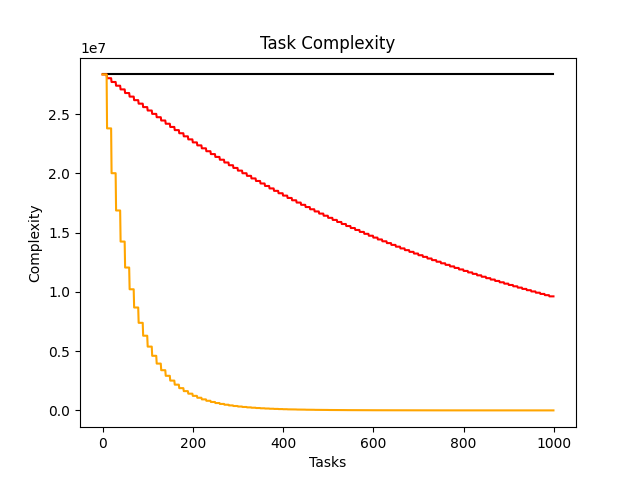
\includegraphics[width= 0.9\columnwidth]{fig/task_complexity.png}\label{fig:use_case_complexity}}
	\hspace*{\fill}    
	\caption[] {\label{fig:use_case_results} Energy expenditure per task: \subref{fig:iso_energy} isolated learning, \subref{fig:itl_energy} incremental+transfer learning,  \subref{fig:cl_energy} collective learning. \subref{fig:use_case_complexity} Scaling of the task complexity.}
\end{figure*}
% ---
The goal of this section is to forecast the energy and resources demand that the robots and AI frameworks in smart factories will have. We also analyze the impact of implementing transfer, incremental and collective learning on this demand. For this, we investigate a prototypical instance of a hypothetical smart factory. This mock factory \hl{is equipped with 10 collaborative robots} whose purpose is to execute a series of tasks, drawn from a pool $ \mathcal{T} $ of industry relevant tasks. In the example we consider \hl{a set of $N_{\mathcal{T}}=1,000$ related and similar tasks}; that is $ \mathcal{T}=\left\lbrace \tau_1,\ldots, \tau_{1000} \right\rbrace$, where we assume $ \tau_i \sim \tau_j $. These tasks will need to be learned by an embodied AI agent so that they can be executed and used in production. We will explore what would be the consequences of the isolated (what we call inefficient) learning paradigm and the envisioned, and arguably desired, collective learning paradigm.

For all the discussed learning types, the initial task complexity is $c_j = 1,600$ episodes. Finally, the power required by \eqref{eq:energy_per_episode} is subdivided as 
% ---
\begin{equation}
    P = P_{BEE}+P_{MIE} + P_{CCE}.
\end{equation}
% ---
To choose $P_{BEE}$, we consider that the smart factory will be populated with state-of-the-art cobots, like the Franka Emika Panda, which requires a typical power of about $\unit[72]{W}$. Furthermore, to approximate $P_{MIE}$, we consider that, in demanding tasks, the power demand of the cobot can go up to a maximum of about $ \unit[300] {W} $. Finally, to determine $P_{CCE}$, we consider that, to overcome the computing effort that learning new tasks will have on the robots' local processors, the smart factory will delegate the computational burden to a remote computing unit (i.e. cloud computing). Thus, we take as reference the work in \cite{Strubell2019EnergyAP}, \hl{where a state-of-the-art machine learning algorithm ({Transformer}$_{base}$) is executed in a cluster, requiring $\unit[1,415.78]{W}$ to solve a task.}

The knowledge transfer effectivity constants are chosen as follows
% ---
\begin{align}\label{eq:transfer_constants}
\begin{split}
    \alpha &=1\times10^{-3}\\
    \beta &=1\times10^{-5}\\
    \gamma &=1\times10^{-7}    
\end{split}
\end{align}
% ---
Finally, we assume that each episode $n$ contains $k=10,000$ iterations.

% Now, assuming in our calculations that all 100 robots, whether in production or in learning, operate 24/7 we have the following numbers:

% SUBSECTION ========================================================================================
\subsection{Isolated learning}
Fig.~\ref{fig:iso_energy} shows the energy demand for a single task. Considering the parameters introduced above, we  estimate the energy and episodes needed by a single robot to learn all $N_{\mathcal{T}}$ tasks. For the episodes, we have
% ---
\begin{equation}
    n^{Iso}_{\mathcal{T}} = N_{\mathcal{T}} \cdot c_j = 1,600\times 10 \times 100 = 1,600,000 \quad\text{episodes}.
\end{equation}
% ---
With $P=\unit[1787.8]{W}$ and using \eqref{eq:energy_per_episode}-\eqref{eq:total_energy}. The total energy equates
% ---
\begin{equation}
    E^{Iso}_{\mathcal{T}} = \unit[283.52]{GJ} %283,520,000,000.0,
\end{equation}
% % ---
 
% ---
% SUBSECTION ========================================================================================
\subsection{Incremental learning and transfer learning}
%For ITL we consider a transfer factor of $\lambda=0.005$ to be used in \eqref{eq:similarity_metric}. Moreover, leveraging parallelization, $m=10$ robots learn $\frac{N_{\mathcal{T}}}{m} = 10$ tasks at the same time. 
Then, using \eqref{eq:complexity_TIL}, \eqref{eq:itl_energy_per_task}, and \eqref{eq:itl_total_energy}; this results in the following episode and energy demands:
% ---
\begin{align}
  n^{ITL}_{\mathcal{T}} &= 972,050\quad\text{episodes} \\
  E^{ITL}_{\mathcal{T}} &= \unit[172.24]{GJ} % 172,247,385,965.70197
\end{align}
% ---
% SUBSECTION ========================================================================================
\subsection{Collective learning in the smart factory: a paradigm change}
While incremental learning only takes the history of one robot into account, collective learning makes it able to use the already learned knowledge of all $m=10$ robots in the collective involved in the learning process. Using eqs. \eqref{eq:complexity_CL}, \eqref{eq:cl_energy_per_task} and \eqref{eq:cl_total_energy}; we obtain the following results,
% ---
\begin{align}
  n^{ITL}_{\mathcal{T}} &= 106,119\quad\text{episodes} \\
  E^{ITL}_{\mathcal{T}} &= \unit[18.80]{GJ} % 18,804,315,849.430477
\end{align}
% ---
This represents energy savings of about $93 \%$ when compared to isolated learning coupled with drastic saving in time as the number of learning episodes reduces considerably. 
 
%  The results for the three schemes are summarized in Table~\ref{tab:results_summary}.
% % ---
% \begin{table}
% \caption{Summary of the results for the learning schemes.\label{tab:results_summary}}
%     \centering
%     \begin{tabular}{c || c | c | c | c}
%          & \multicolumn{2}{c|}{single robot} & \multicolumn{2}{|c}{multiple robots} \\
%          & $E_{\mathcal{T}}\quad[GJ]$ & $n\quad [\#]$ & $E_\mathcal{T} [GJ]$ & $n \quad[\#]$ \\
%         \hline
%         \hline
%         IL & $56.57$ & $160,000$ & $283.52$ & $1,600,000$ \\
%         \hline
%         ITL & --- & --- & $172.24$ & $972,050$ \\
%         \hline
%         CL & --- & --- & $18.80$ & $106,119$ \\
%         \hline
%     \end{tabular}
% \end{table}
% ---

The energy demands as the number of learned tasks increases for all the considered learning schemes is shown in  Fig.~\ref{fig:use_case_results}. Evidently, collective learning reduces the energy consumption to the minimum in the least number of trial episodes. Furthermore, Fig.~\ref{fig:use_case_complexity} shows the scaled down complexities considering the parameters in \eqref{eq:transfer_constants}.

